\section{Importing scenes}
This section shows an example on how a scene can be imported into Mitsuba.
We will start with the 3ds max file contained in \texttt{kitchen\_clean\_pomesuba.rar}, which can be obtained from \texttt{http://ompf.org/vault}.
Interaction with other programs, such as Maya, Blender or SketchUp is supported using similar approaches as the one described here.
Begin by opening the file in 3ds max:
\begin{center}
\scalebox{.4}{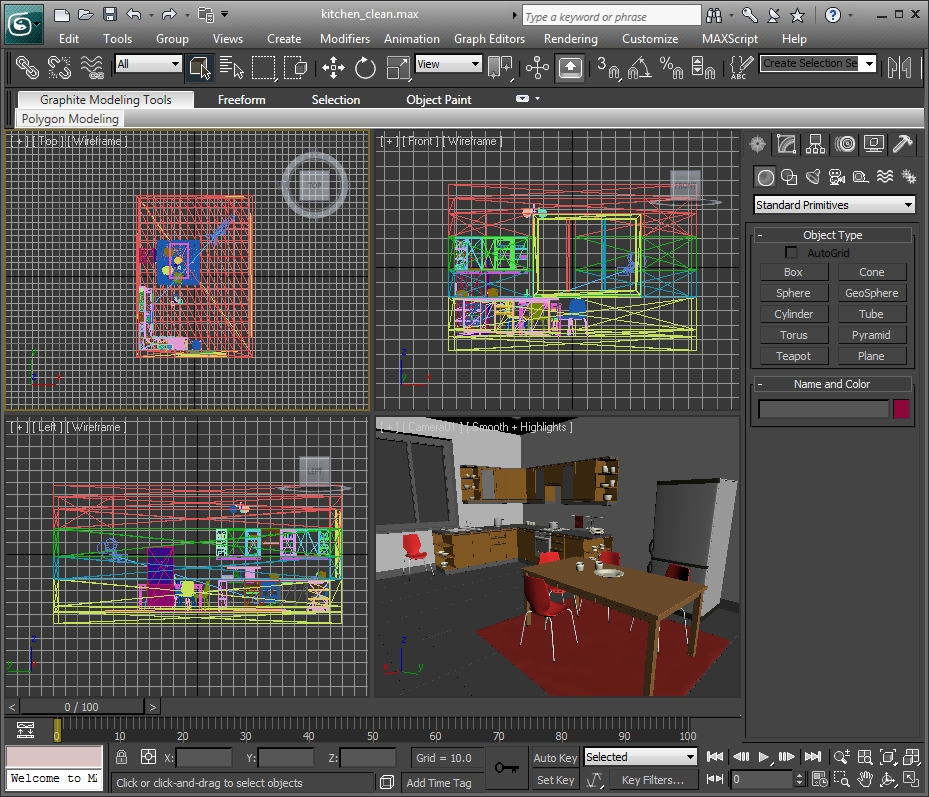
\includegraphics{images/import_1.jpg}}
\end{center}
Go to File$\to$Export$\to$Export, enter a filename for the exported scene and choose "Autodesk Collada (*.DAE)" as the target file type.
In the upcoming dialog, make sure that `Single Matrix' is disabled at the bottom -- otherwise your camera will face into the 
wrong direction (this is only an issue with Autodesk products).
\begin{center}
\scalebox{.4}{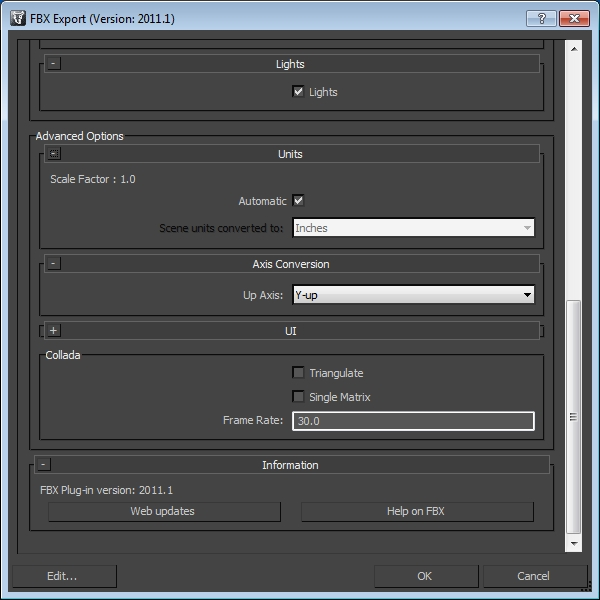
\includegraphics{images/import_2.jpg}}
\end{center}
Launch Mitsuba and select File$\to$Import. Next, open the exported DAE file by clicking on the topmost browse button and and change the color format to sRGB. The remaining options can be ignored for now.
\begin{center}
\scalebox{.5}{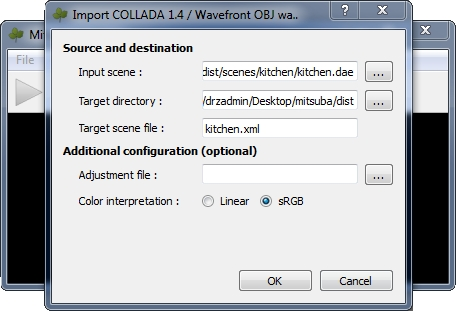
\includegraphics{images/import_3.jpg}}
\end{center}
After a moment, the scene will open -- rendering it in this form, e.g. using path tracing will produce an image like this:
\begin{center}
\scalebox{.5}{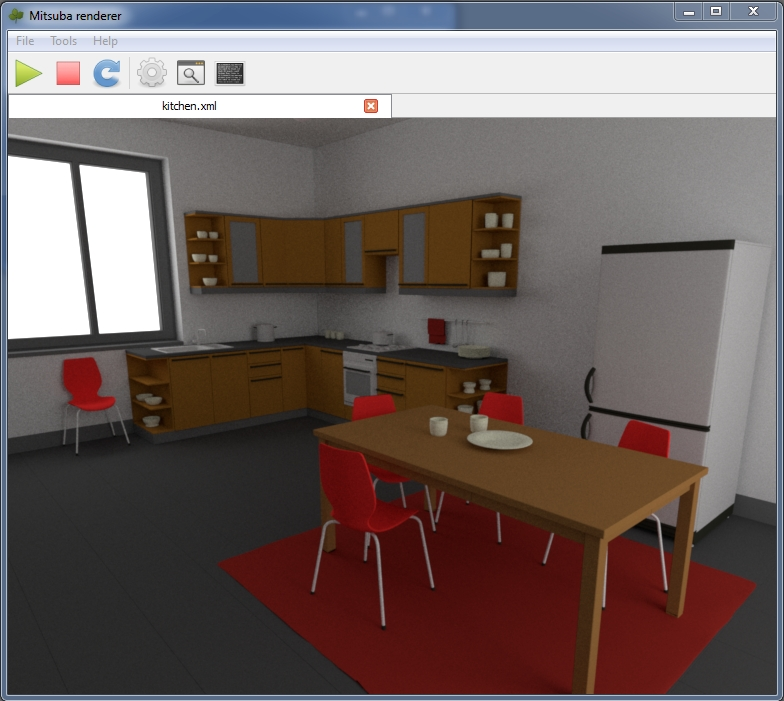
\includegraphics{images/import_4.jpg}}
\end{center}
Many of the materials in this rendering are incorrect, which is in part caused by the limited material description abilities of COLLADA.
To fix them, we will have to provide a so-called adjustment file. The idea here is very simple: if you look at the output file (\texttt{kitchen.xml}) 
generated by the conversion, you will notice that every relevant XML node has an \code{id} attribute. For instance, there is a material named \code{glass} with the following entry:
\begin{xml}
<bsdf id="glass" type="diffuse">
	<rgb name="reflectance" value="0.588235 0.588235 0.588235"/>
</bsdf>
\end{xml}
\newpage
This is the reason why the glass looks incorrect in the above rendering: it is completely diffuse!
To fix it, we will provide a dielectric material with the same \code{id} attribute, which then allows Mitsuba
to replace the incorrect material during import.
We can do this by creating a file named \code{kitchen\_adjustments.xml} containing
the following lines:
\begin{xml}
<adjustments>
	<bsdf id="glass" type="dielectric"/>
</adjustments>
\end{xml}
The adjustments mechanism can also be used to add content, such as light sources or even geometry. Insert the objects which should
be part part of the scene into the adjustment file, and they will be copied on every import. Replacement is not limited to materials -- it
can also be applied to the integrator or the camera -- you only have to make sure that the \code{id} fields match for the replacement to happen.

After tweaking the remaining materials in this fashion, it is possible to re-import the scene and this time specify the adjustment file in the import dialog.
This makes it possible to get the following more realistic result (material descriptions courtesy of Pomesuba):
\begin{center}
\scalebox{.32}{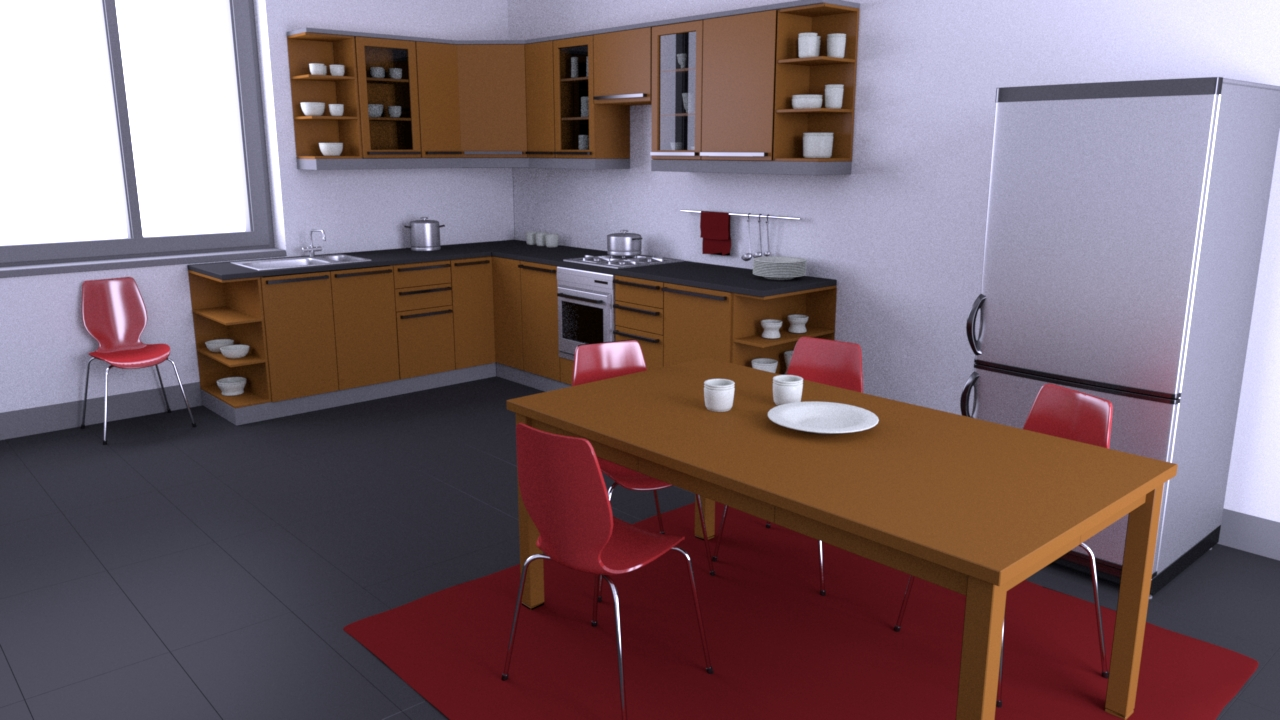
\includegraphics{images/import_5.jpg}}
\end{center}
When modeling scenes that should later be rendered in Mitsuba, it is
important to keep in mind that physically based rendering systems are by
principle incompatible with many of the options provided in today's 
modeling toolkits. Hence, one should refrain from using features such 
\begin{itemize}
\item adjusting the amount of ambient occlusion on an object 
\item using an ambient reflection term
\item selectively enabling/disabling light sources for certain
objects
\item using point/spot lights with anything other than a quadratic falloff
\item creating materials, which reflect more light than they receive
\end{itemize}
This is only a partial list --- if in doubt, ask yourself whether a feature
is physically plausible before using it.
